\documentclass{beamer}

\usepackage{amsmath, amssymb}
\usepackage{tikz-cd}
\usepackage{xcolor}
\usepackage{graphicx}
\usepackage{capt-of}

\title{MAT434: Theory of Mathematical Statistics - Joint Distributions}
\subtitle{Independent Random Variables \cite{RJA2006}}
\author{\textbf{Miraj Samarakkody}}
\institute{Tougaloo College}
\date{Updated: \today}

\begin{document}

\begin{frame}
    \titlepage
\end{frame}




\begin{frame}{Independent Random Variables}
    \begin{block}{Definition}
        Random variables \(X_1,X_2, X_3, \dots, X_n\) are said to be \textit{independent} if their joint cdf factors into the product of their marginal cdf's:
        \[F(x_1, x_2, \dots, x_n)= F_{X_1}(x_1)F_{X_2}(x_2)\dots F_{X_n}(x_n)\] for all \(x_1, x_2, \dots, x_n\). 
    \end{block}\pause
    \vspace{0.5cm}  

    This definition holds for both continuous and discrete random variables:\pause
    \begin{itemize}
        \item For discrete random variables, it is equivalent to their joint frequency function factors.\pause
        \item For continuous random variables, it is equivalent to their joint density fuction factors. 
    \end{itemize}
\end{frame}

\begin{frame}{}
    If \(X\) and \(Y\) are independent, then \[P(X \in A, Y \in B) = P(X \in A)P(Y \in B)\]
\end{frame}

\begin{frame}
    \frametitle{Example A}

    Suppose that the point \((X,Y)\) is uniformly distributed on the square 
    \[S= \{(x,y)| -1/2 \leq x \leq 1/2, -1/2 \leq y \leq 1/2\}\]
    \[f_{XY}(x,y)=\begin{cases}
        1 & \text{for } (x,y) \in S\\
        0 & \text{otherwise}
    \end{cases}\]
    
    Prove that \(X\) and \(Y\) are independent.

\end{frame}

\begin{frame}
    \frametitle{Example B}
Now consider rotating the square by \(45^{\circ}\) to obtain the diamond shape.

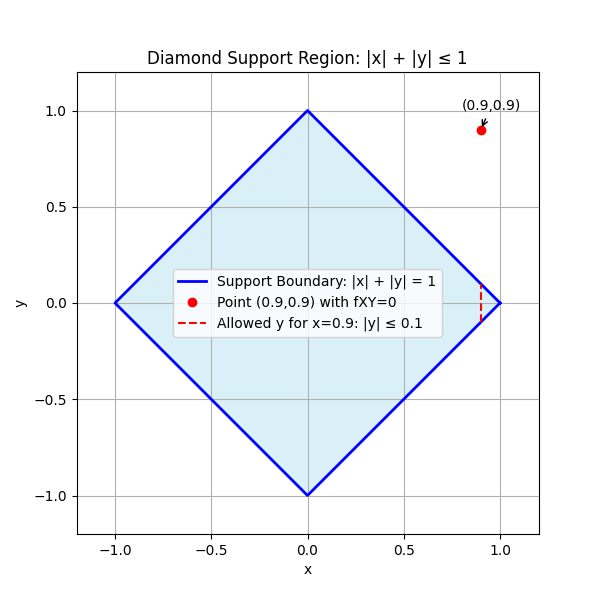
\includegraphics[scale=0.5]{Figures/fig_10.png}
\end{frame}
\begin{frame}
    \frametitle{References}
    \bibliographystyle{plain} % or another style like unsrt, alpha, etc.
    \bibliography{references}  % omit the .bib extension
\end{frame}



\end{document}